\problemname{kcuD dlanoD}
Oh no! Donald Duck accidentally went through Professor Ludwig von Drake’s reversing machine, so now everything he sees is mirror inverted.

Quack-it, this was very untimely. Scrooge McDuck namely has a very important quest for Donald Duck. He needs Donald to choose the biggest out of two money bags so that he, Mr. McDuck, can become even richer than he already is.

\begin{figure}[!h]
\begin{center}
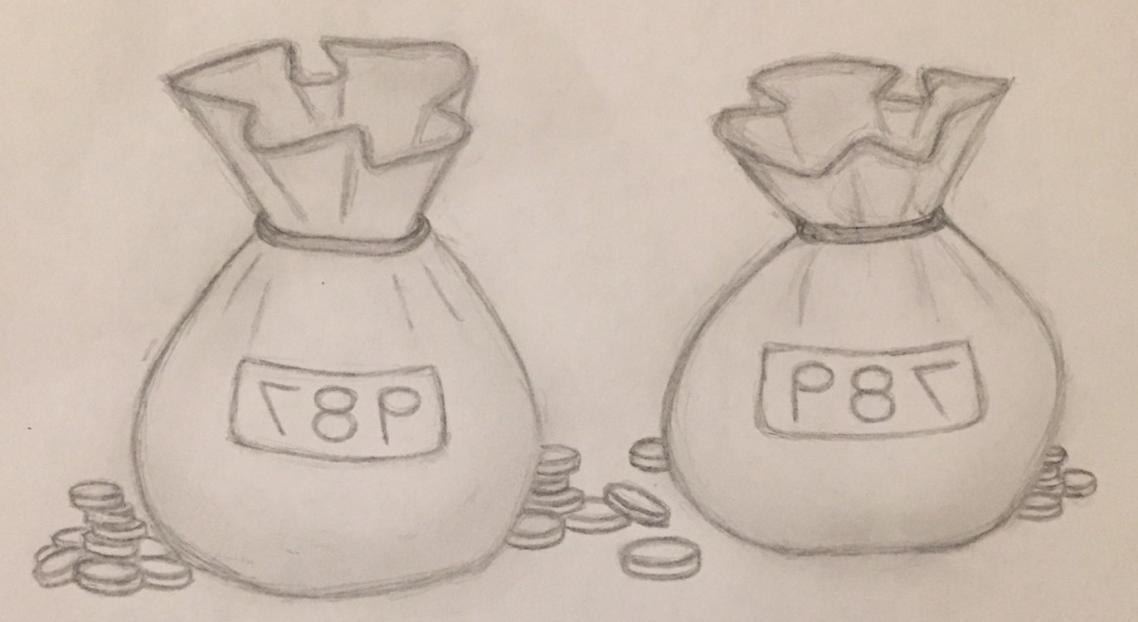
\includegraphics[width=0.5\textwidth]{moneybags.jpg}
\end{center}
\end{figure}

In order to not make his uncle furious, Donald Duck has asked you for help. He will give you the two
mirror inverted numbers he sees on the two money bags. Your task is to help him choose the biggest
of these numbers. Print \texttt{1} if Donald should choose the first number and \texttt{2} if he should choose the
second number. Keep in mind: The mirror reversal has made Donald see twos as fives and fives as twos.
Otherwise Donald Duck will see the digits as they are, but in reversed order. The bags don't
contain the same amount of money and the numbers on the bags neither start nor end with a zero.

\section*{Input}
The input consists of a single line with two space-separated integers $N$ and $M$ ($1
\leq N, M < 10^6$)

\section*{Output}
Output \texttt{1} if the first bag has more money, or \texttt{2} if the second bag has more.
